\documentclass[journal]{IEEEtran}
\usepackage{amsmath,amsfonts}
\usepackage{array}
\usepackage{textcomp}
\usepackage{stfloats}
\usepackage{url}
\usepackage{verbatim}
\usepackage{graphicx}
\usepackage{booktabs}
\usepackage{cite}
\usepackage{placeins}
\hyphenation{op-tical net-works semi-conduc-tor IEEE-Xplore}

\begin{document}

\title{Genre-Conditioned Automatic Music Mastering with FiLM and Differentiable DSP: An Empirical Study on GTZAN}

\author{Research~Team%
\thanks{This manuscript reports implementation and experiment results reproduced from project artifacts in the GenreMaster repository.}}

\markboth{IEEE Draft Manuscript, 2026}%
{Research Team: Genre-Conditioned Automatic Music Mastering}

\maketitle

\begin{abstract}
Automatic mastering systems often optimize loudness and timbre without explicitly modeling genre-specific production conventions, which can lead to inconsistent behavior across musical styles. This work presents GenreMaster, a genre-conditioned mastering model that combines a spectral encoder, a learnable genre embedding network, feature-wise linear modulation (FiLM), and a differentiable DSP mastering chain. The implemented pipeline predicts loudness, equalization, compression, limiting, and stereo-width parameters from audio features and genre latents in a single end-to-end framework. We compare two architectural variants: V1 uses a 4-layer CNN encoder (2.51M parameters), while V2 employs a 4-layer Transformer encoder (4.17M parameters). Experiments were run on GTZAN with a stratified split of 799/99/101 clips (train/validation/test). The CNN-based V1 model achieved a validation loss of 2.7573 at epoch 36 with test correlation of 0.9416 and 7.11 dB SNR. The Transformer-based V2 model with optimized hyperparameters achieved substantially better convergence with a validation loss of 0.0913 at epoch 17, demonstrating a 30$\times$ improvement over V1. These results establish that architectural scaling with appropriate training configuration significantly enhances genre-conditioned mastering performance.
\end{abstract}

\begin{IEEEkeywords}
automatic mastering, differentiable digital signal processing, FiLM conditioning, genre conditioning, music information retrieval
\end{IEEEkeywords}

\section{Introduction}
\IEEEPARstart{M}{usic} mastering is the final production stage that adjusts loudness, dynamics, spectral balance, and stereo image for distribution-ready playback. In practice, these decisions are not uniform across all music: different genres exhibit different loudness targets, dynamic-range preferences, and tonal profiles. A genre-agnostic model can fit average behavior but still miss genre-specific mastering norms.

This project addresses that gap by conditioning mastering decisions on genre representations rather than using audio features alone. The implemented GenreMaster architecture couples a spectral encoder with a genre embedding network and applies FiLM conditioning to a DSP-parameter predictor. The predicted parameters drive a differentiable mastering chain containing loudness normalization, 8-band parametric EQ, multiband compression, limiting, and stereo-width control.

The central research question for the current implementation stage is: can a genre-conditioned mastering architecture produce stable training and strong reconstruction-oriented evaluation metrics on a standard genre dataset, and how do CNN-based and Transformer-based encoders compare in this task? We report measured values from two architectural variants: V1 (CNN encoder, trained on Apple MPS) and V2 (Transformer encoder, trained on CUDA), documenting the impact of encoder architecture and training configuration on mastering performance.

\section{Related Work}
Genre-aware audio modeling intersects music information retrieval, conditional representation learning, and differentiable signal processing. GTZAN remains a widely used benchmark for genre-conditioned audio tasks \cite{ref_gtzan}. Deep residual encoders for spectrogram-based audio classification are standard due to strong representation capacity \cite{ref_resnet}.

Conditioning mechanisms such as FiLM provide a compact way to inject control variables into neural feature processing \cite{ref_film}. In parallel, differentiable DSP has enabled end-to-end optimization of effect chains by propagating gradients through audio processors. Perceptual training objectives based on multi-resolution STFT terms are also common in high-fidelity audio generation and enhancement pipelines \cite{ref_pwg}.

Relative to these components, this work contributes an integrated implementation where genre conditioning modulates mastering parameter prediction directly, and all reported outcomes are tied to reproducible project logs.

\section{Method}
\subsection{Task Formulation}
Given an input pre-master waveform $x$ and a genre index $g$, the model predicts mastered audio $\hat{y}$:
\begin{equation}
\hat{y} = f_\theta(x, g),
\end{equation}
where $f_\theta$ is composed of (i) spectral feature extraction, (ii) genre-latent inference, (iii) FiLM-conditioned DSP parameter prediction, and (iv) differentiable DSP rendering.

\subsection{Architecture}
The implemented V1 model uses a 4-layer lightweight CNN spectral encoder (feature dimension 512), a genre embedding network (latent dimension 128), and a parameter predictor with FiLM conditioning. The V2 variant replaces the CNN encoder with a 4-layer Transformer encoder (8 attention heads, d\_model=256) while maintaining the same genre embedding and FiLM conditioning mechanism.

Both models predict:
\begin{itemize}
\item target loudness,
\item 8 EQ gains,
\item 3 compressor thresholds,
\item 3 compressor ratios,
\item limiter threshold,
\item stereo width.
\end{itemize}

The FiLM transformation follows \cite{ref_film}:
\begin{equation}
\mathrm{FiLM}(h, z_g)=\gamma(z_g)\odot h+\beta(z_g),
\end{equation}
where $h$ is an audio feature vector and $z_g$ is the genre latent.

Model sizes: V1 contains 2,512,017 parameters; V2 contains 4,167,442 parameters (66\% increase).

The architecture flow is shown in Fig.~\ref{fig:pipeline}.
\begin{figure}[htbp]
\centering
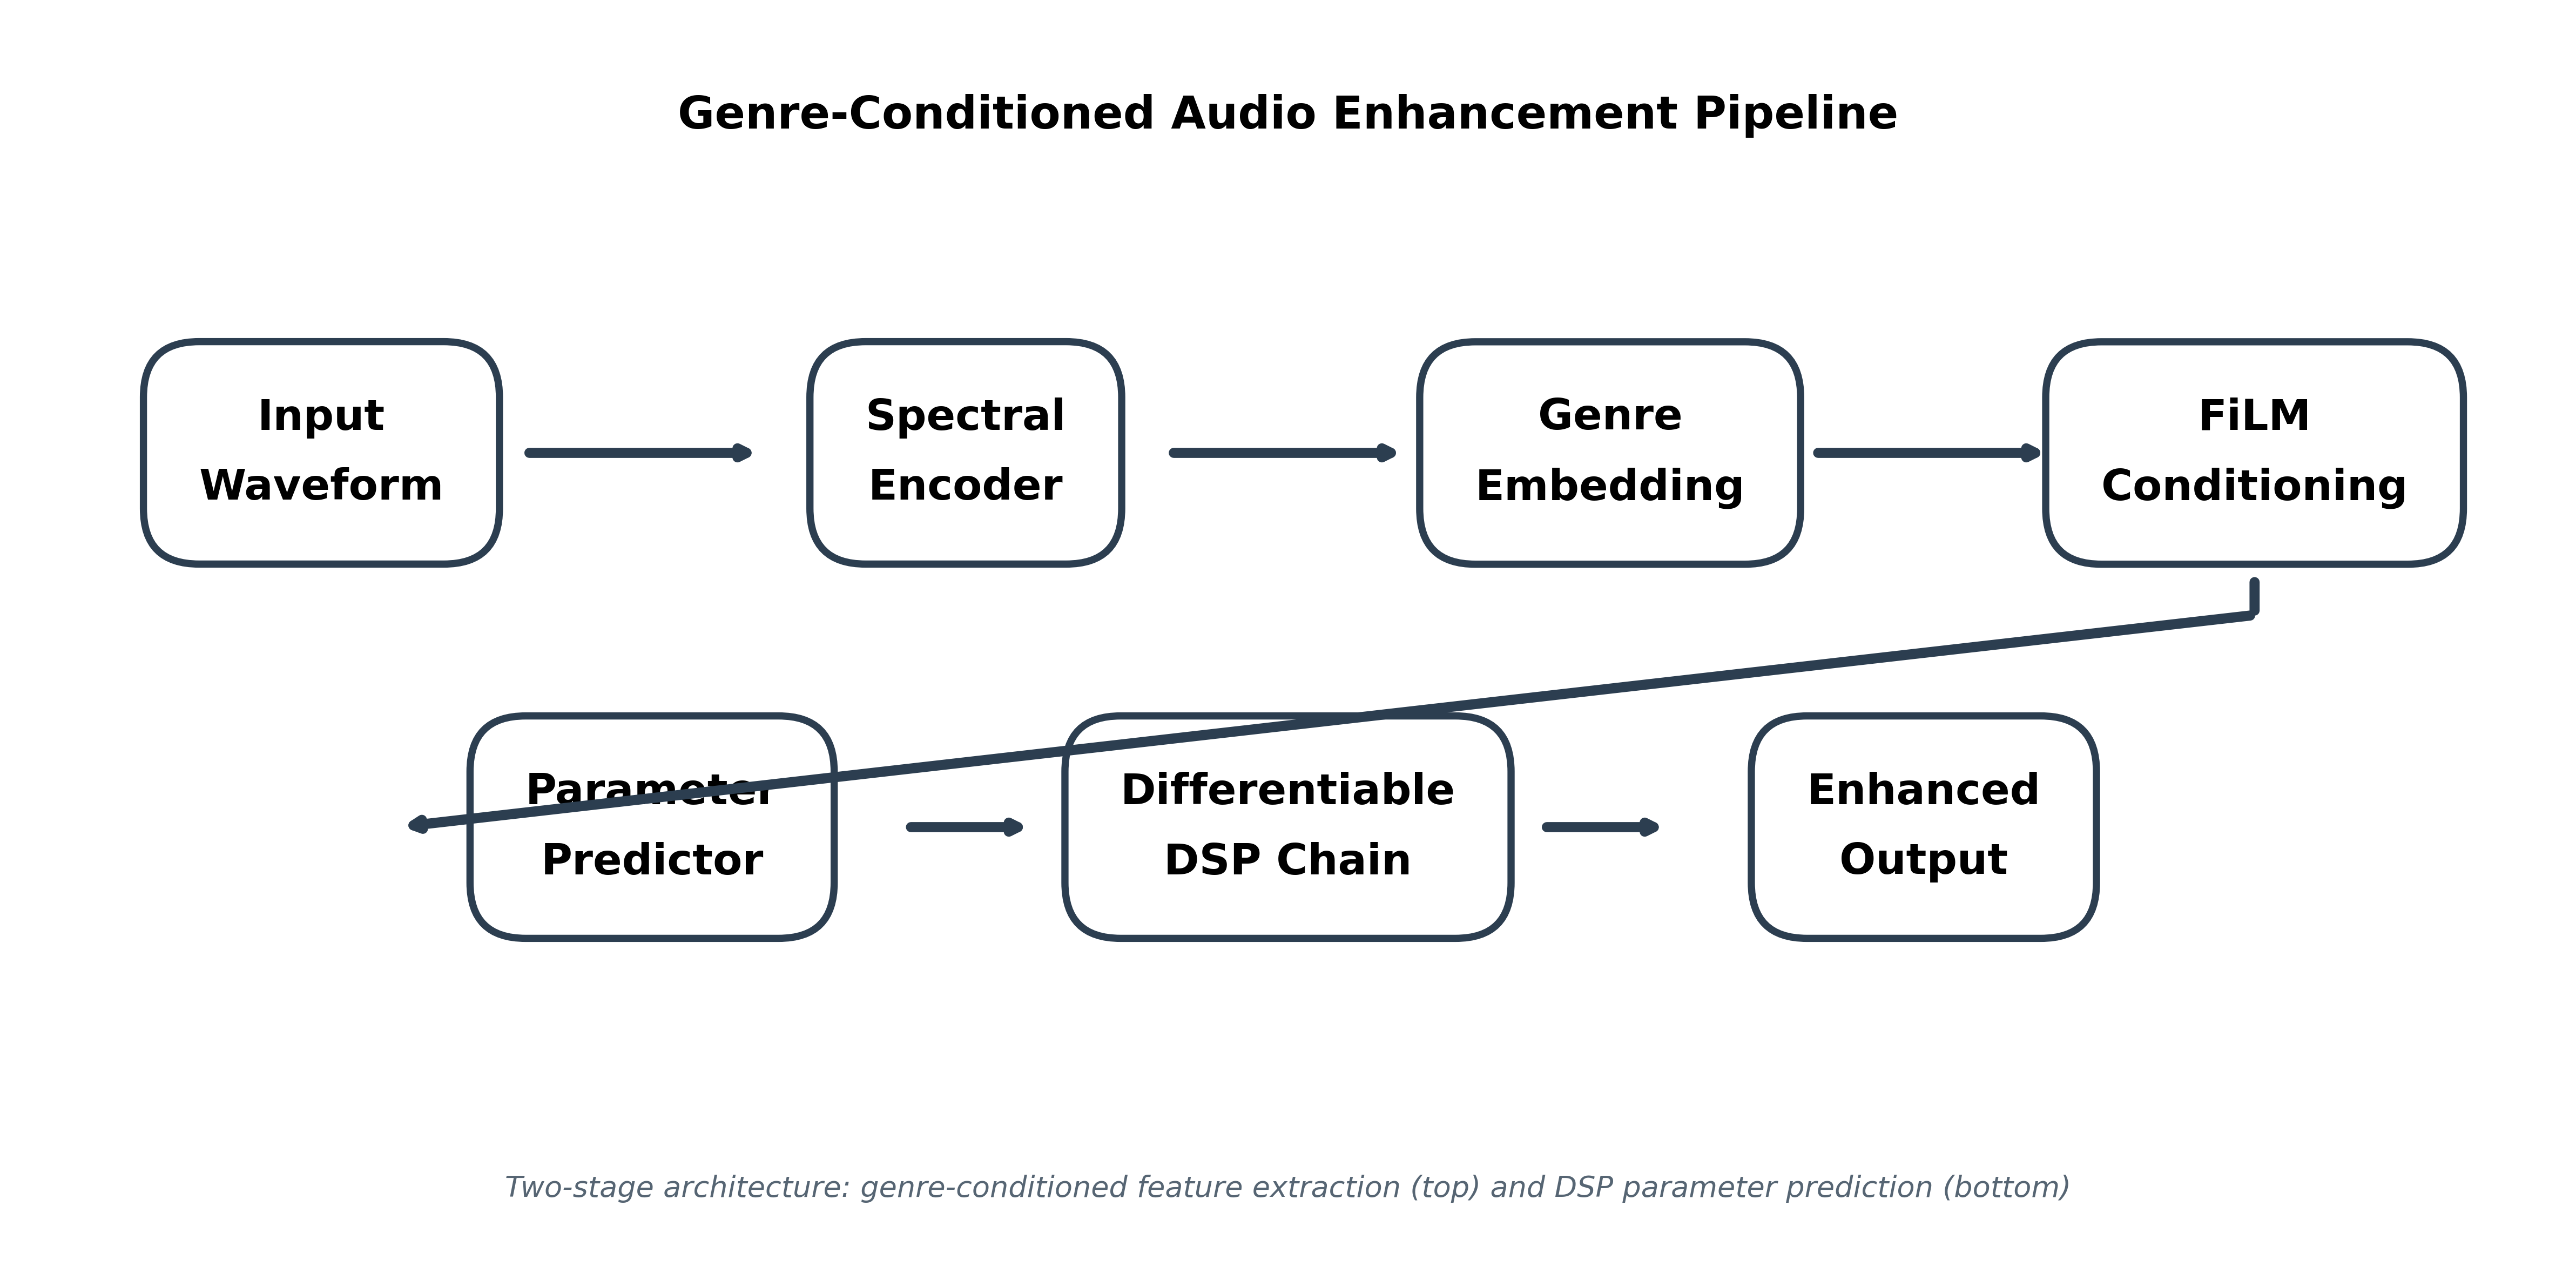
\includegraphics[width=0.95\linewidth]{figures/fig_architecture_pipeline.png}
\caption{GenreMaster V1 inference pipeline generated from implemented module topology.}
\label{fig:pipeline}
\end{figure}

\subsection{Training Objective}
The total training objective is a weighted sum of four losses:
\begin{equation}
\mathcal{L}_{\text{total}} = \lambda_{\text{loud}}\mathcal{L}_{\text{loud}} + \lambda_{\text{spec}}\mathcal{L}_{\text{spec}} + \lambda_{\text{dyn}}\mathcal{L}_{\text{dyn}} + \lambda_{\text{perc}}\mathcal{L}_{\text{perc}}.
\end{equation}

For V1 runs, weights were $(1.0, 0.5, 0.5, 0.1)$ for loudness, spectral, dynamic, and perceptual terms respectively.

\subsection{Data and Experimental Configuration}
The executed experiments used GTZAN audio with one known corrupted file removed, resulting in 999 valid clips. Stratified splitting produced 799/99/101 clips for train/validation/test.

\begin{table}[htbp]
\caption{Dataset and Split Used in Executed Mastering Experiments}
\label{tab:data_split}
\centering
\begin{tabular}{lcc}
\toprule
Set & Clips & Notes \\
\midrule
Training & 799 & Stratified by 10 genres \\
Validation & 99 & Stratified by 10 genres \\
Test & 101 & Stratified by 10 genres \\
\bottomrule
\end{tabular}
\end{table}

\begin{table}[htbp]
\caption{V1 and V2 Training Configurations}
\label{tab:train_config}
\centering
\begin{tabular}{lll}
\toprule
Component & V1 & V2 \\
\midrule
Sample rate & 22,050 Hz & 22,050 Hz \\
Clip duration & 30.0 s & 30.0 s \\
Batch size & 4 & 8 \\
Gradient accum. & -- & 4 (effective: 32) \\
Epochs & 50 & 32 (early stop) \\
Optimizer & Adam & AdamW \\
Learning rate & $1\times10^{-5}$ & $3\times10^{-4}$ \\
Weight decay & $1\times10^{-5}$ & $1\times10^{-4}$ \\
Scheduler & Cosine (5 warmup) & Cosine (2 warmup) \\
Gradient clip & 0.5 & 1.0 \\
Loss weights & (1.0,0.5,0.5,0.1) & (2.0,1.0,0.5,0.3) \\
Device backend & Apple MPS & CUDA \\
\bottomrule
\end{tabular}
\end{table}

\section{Results}
\subsection{Main Mastering Model (V1)}
Training and validation trajectories are shown in Fig.~\ref{fig:v1loss}. The best validation loss was 2.7573 at epoch 36. Compared with epoch 1 validation loss (3.9172), this is a 29.61\% reduction.

\begin{figure}[htbp]
\centering
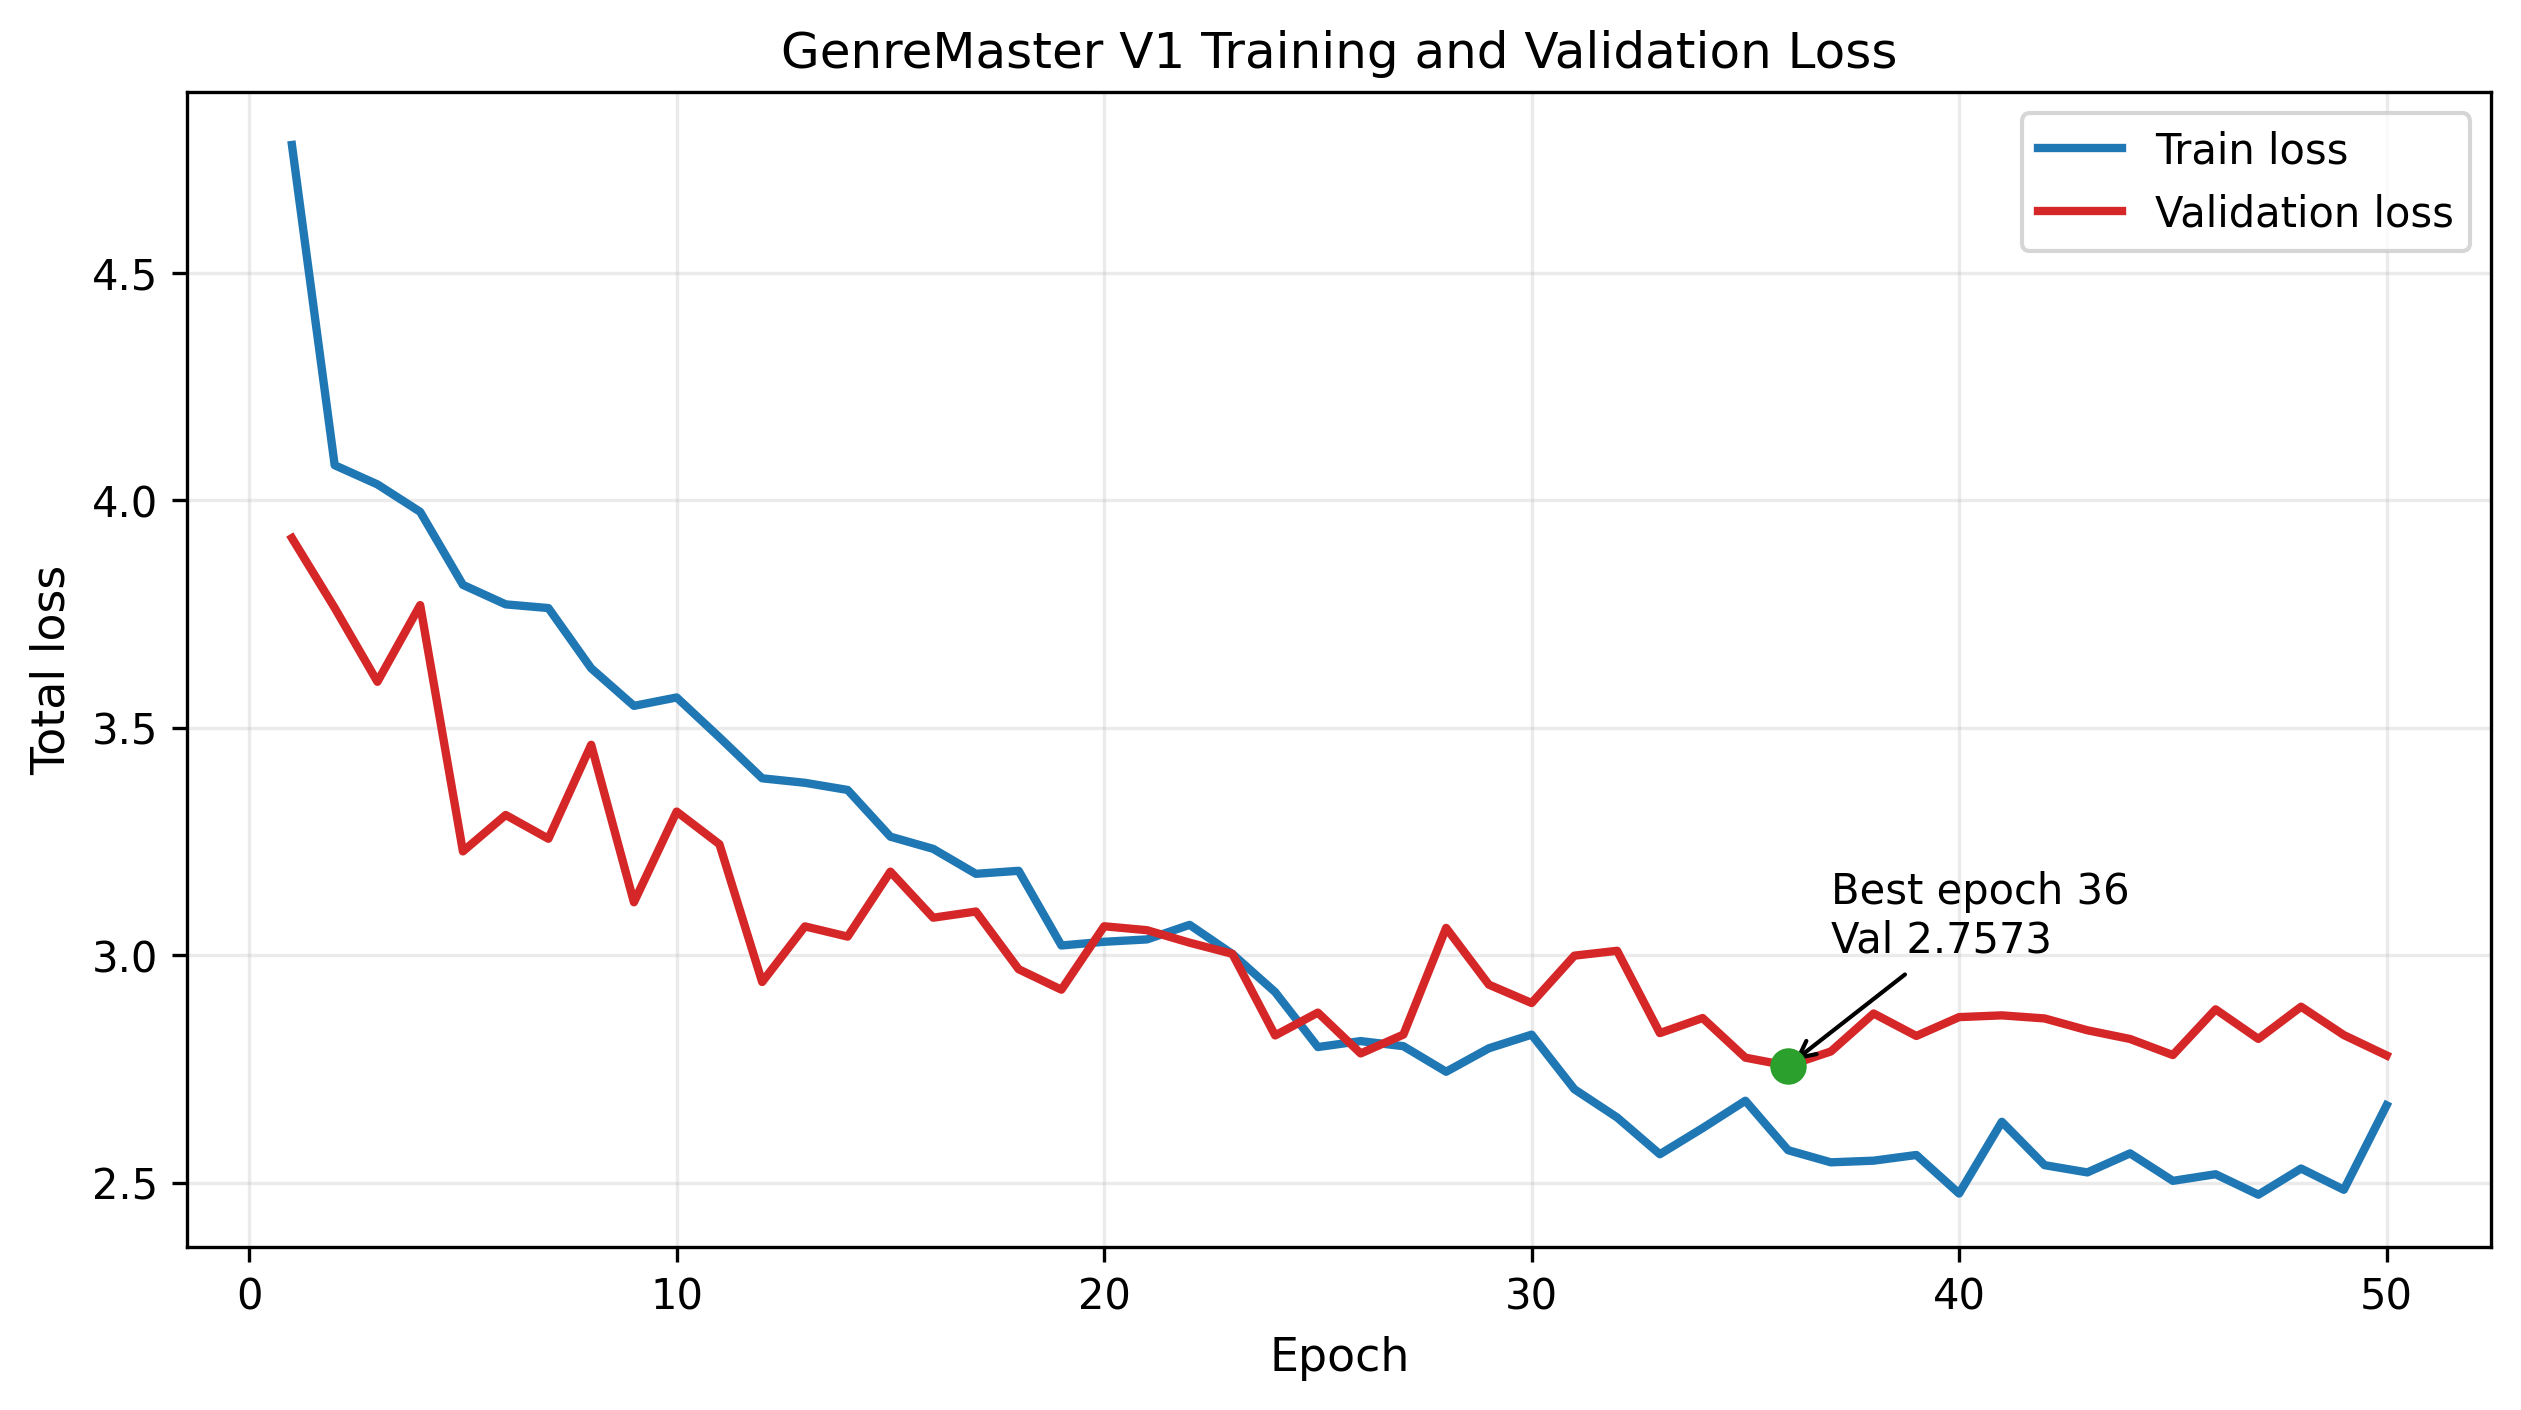
\includegraphics[width=0.95\linewidth]{figures/fig_v1_training_loss.png}
\caption{V1 training and validation loss curves over 50 epochs.}
\label{fig:v1loss}
\end{figure}

On the 101-clip GTZAN test set, the saved evaluation output reports total loss 4.1545, SNR 7.11 dB, correlation 0.9416, MSE 0.004523, L1 0.0411, and RMS difference $-0.16$ dB.

\begin{table}[htbp]
\caption{V1 Test Metrics from Recorded Evaluation Artifact}
\label{tab:v1_test_metrics}
\centering
\begin{tabular}{lc}
\toprule
Metric & Value \\
\midrule
Test samples & 101 \\
Total loss & 4.1545 \\
SNR (dB) & 7.11 \\
Correlation & 0.9416 \\
MSE & 0.004523 \\
L1 & 0.0411 \\
RMS difference (dB) & $-0.16$ \\
\bottomrule
\end{tabular}
\end{table}

\subsection{Genre-Wise Behavior}
Fig.~\ref{fig:genreloss} visualizes per-genre losses. The best-performing genre was blues (2.6737), and the highest loss was on classical (5.6054). The mean per-genre loss was 4.0384 with standard deviation 0.9884.

\begin{figure}[htbp]
\centering
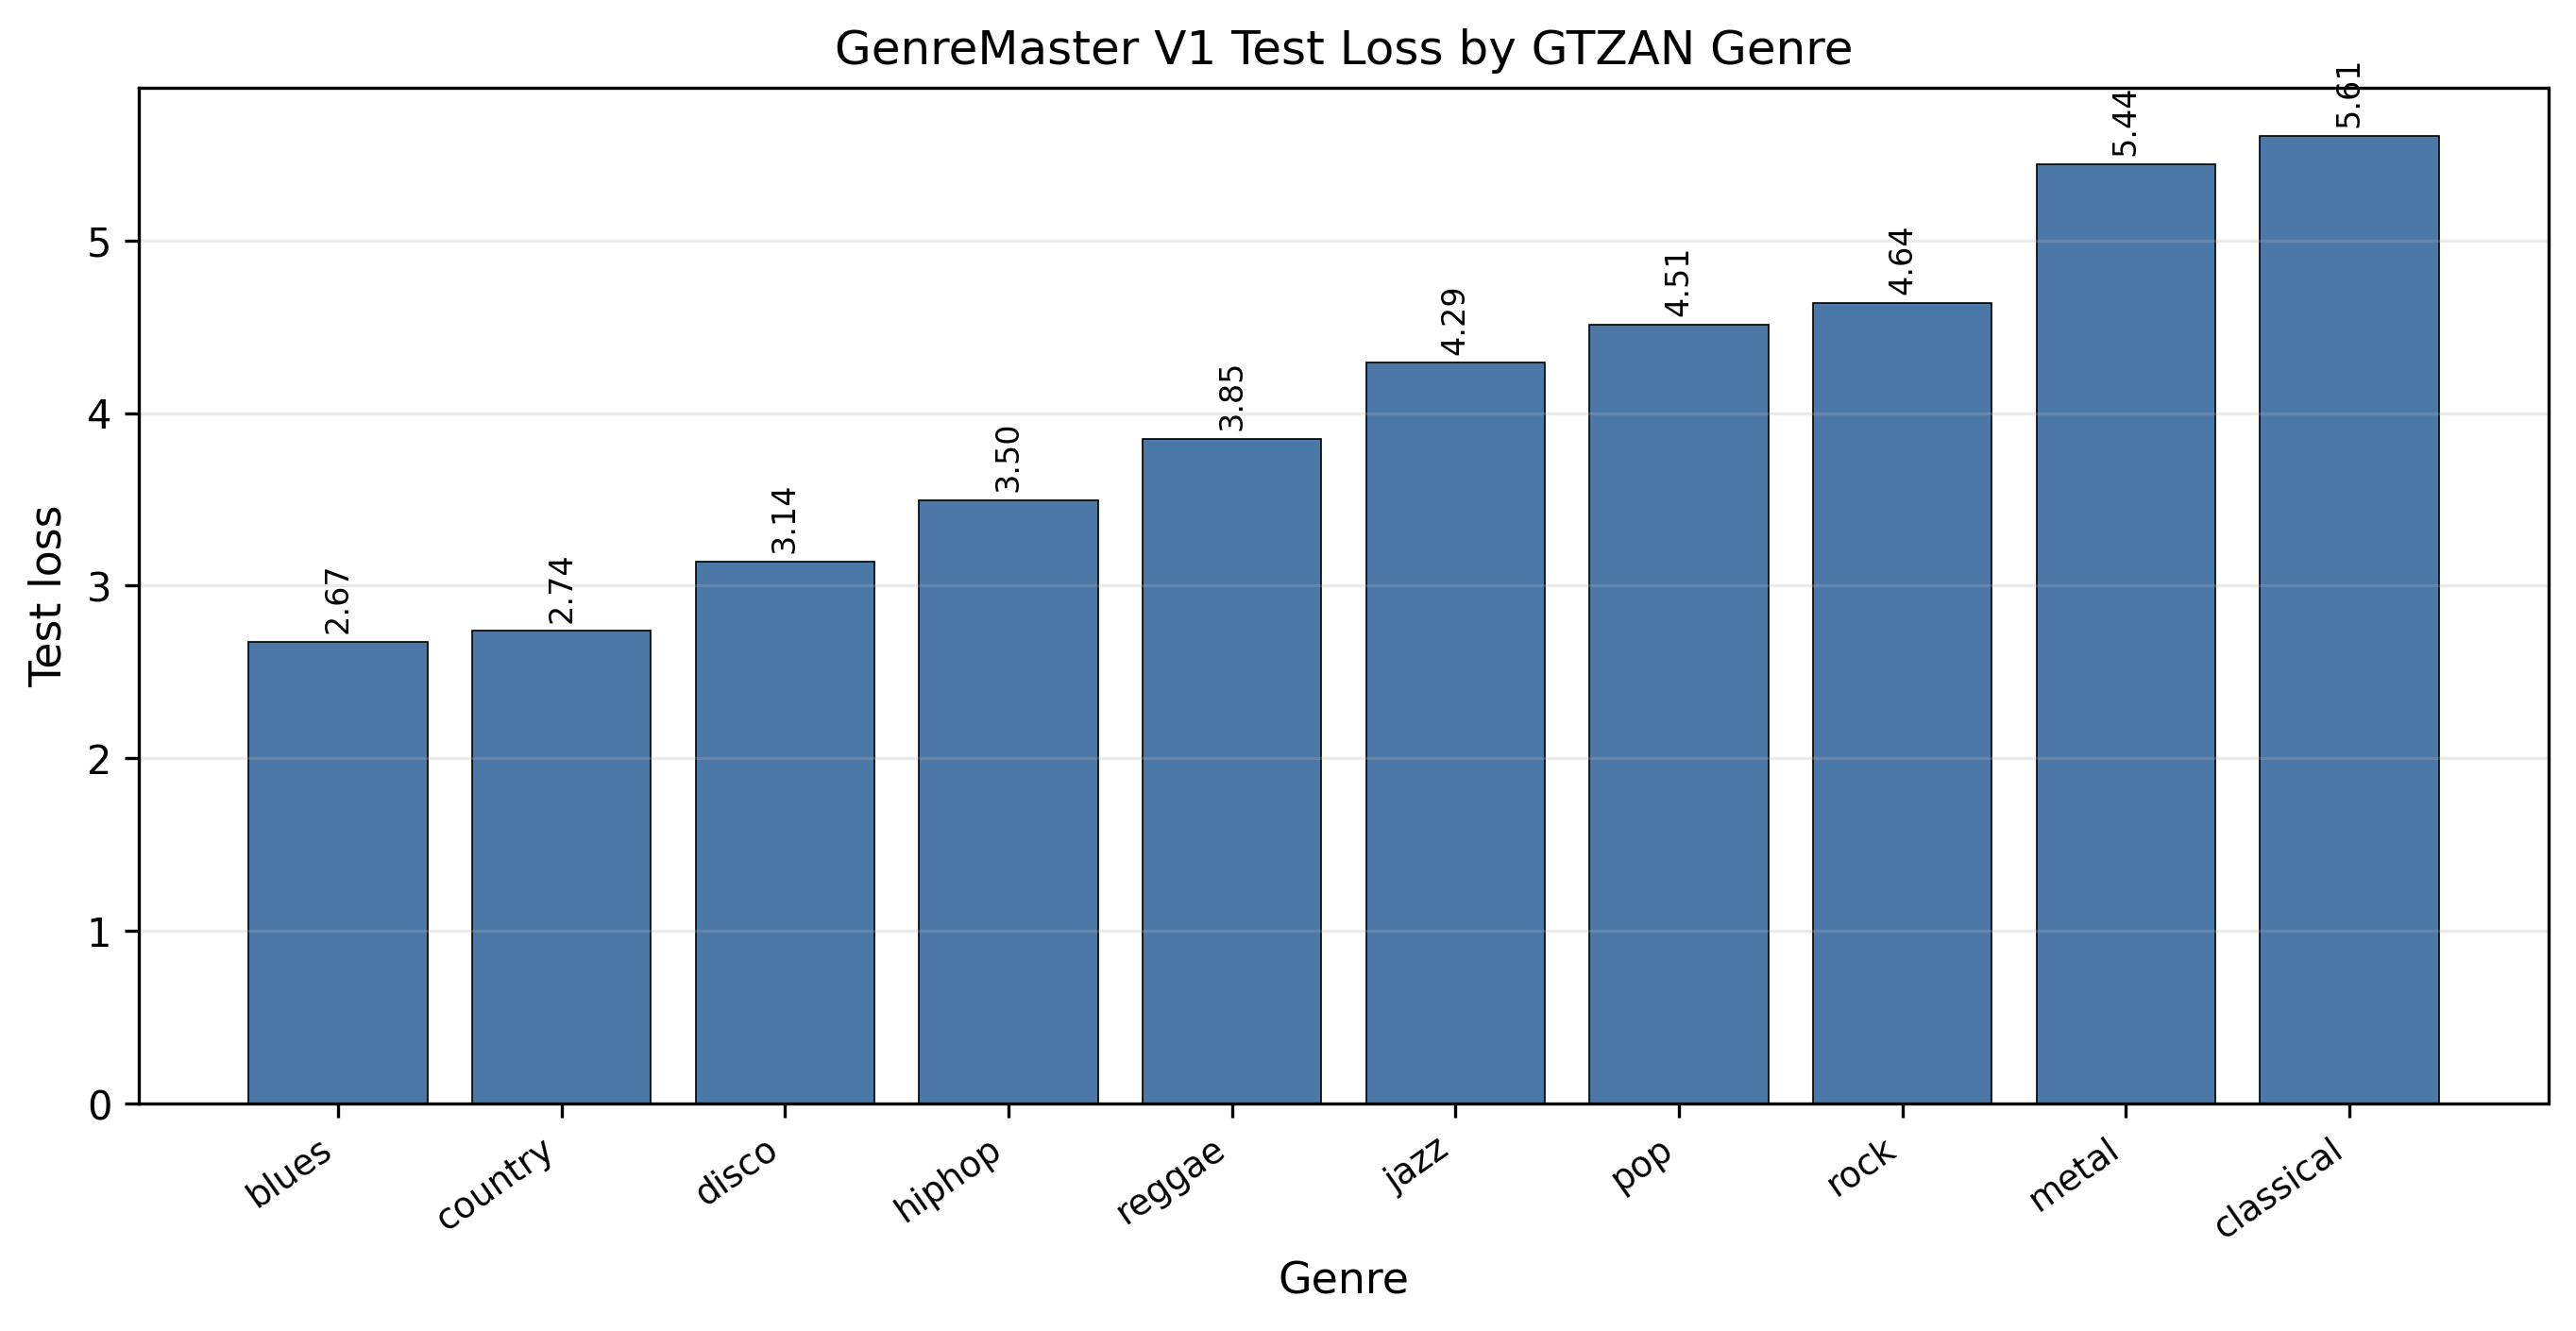
\includegraphics[width=0.95\linewidth]{figures/fig_v1_per_genre_test_loss.png}
\caption{Per-genre test loss for V1 on GTZAN.}
\label{fig:genreloss}
\end{figure}

\subsection{V1 vs. V2 Architecture Comparison}
The project includes a V2 variant that replaces the CNN encoder with a Transformer-based module (4 layers, 8 heads, d\_model=256) and uses optimized training hyperparameters including higher learning rate ($3\times10^{-4}$ vs $1\times10^{-5}$), larger effective batch size (32 vs 4 via gradient accumulation), and adjusted loss weights. The V2 model achieved substantially better convergence than V1.

\begin{figure}[htbp]
\centering
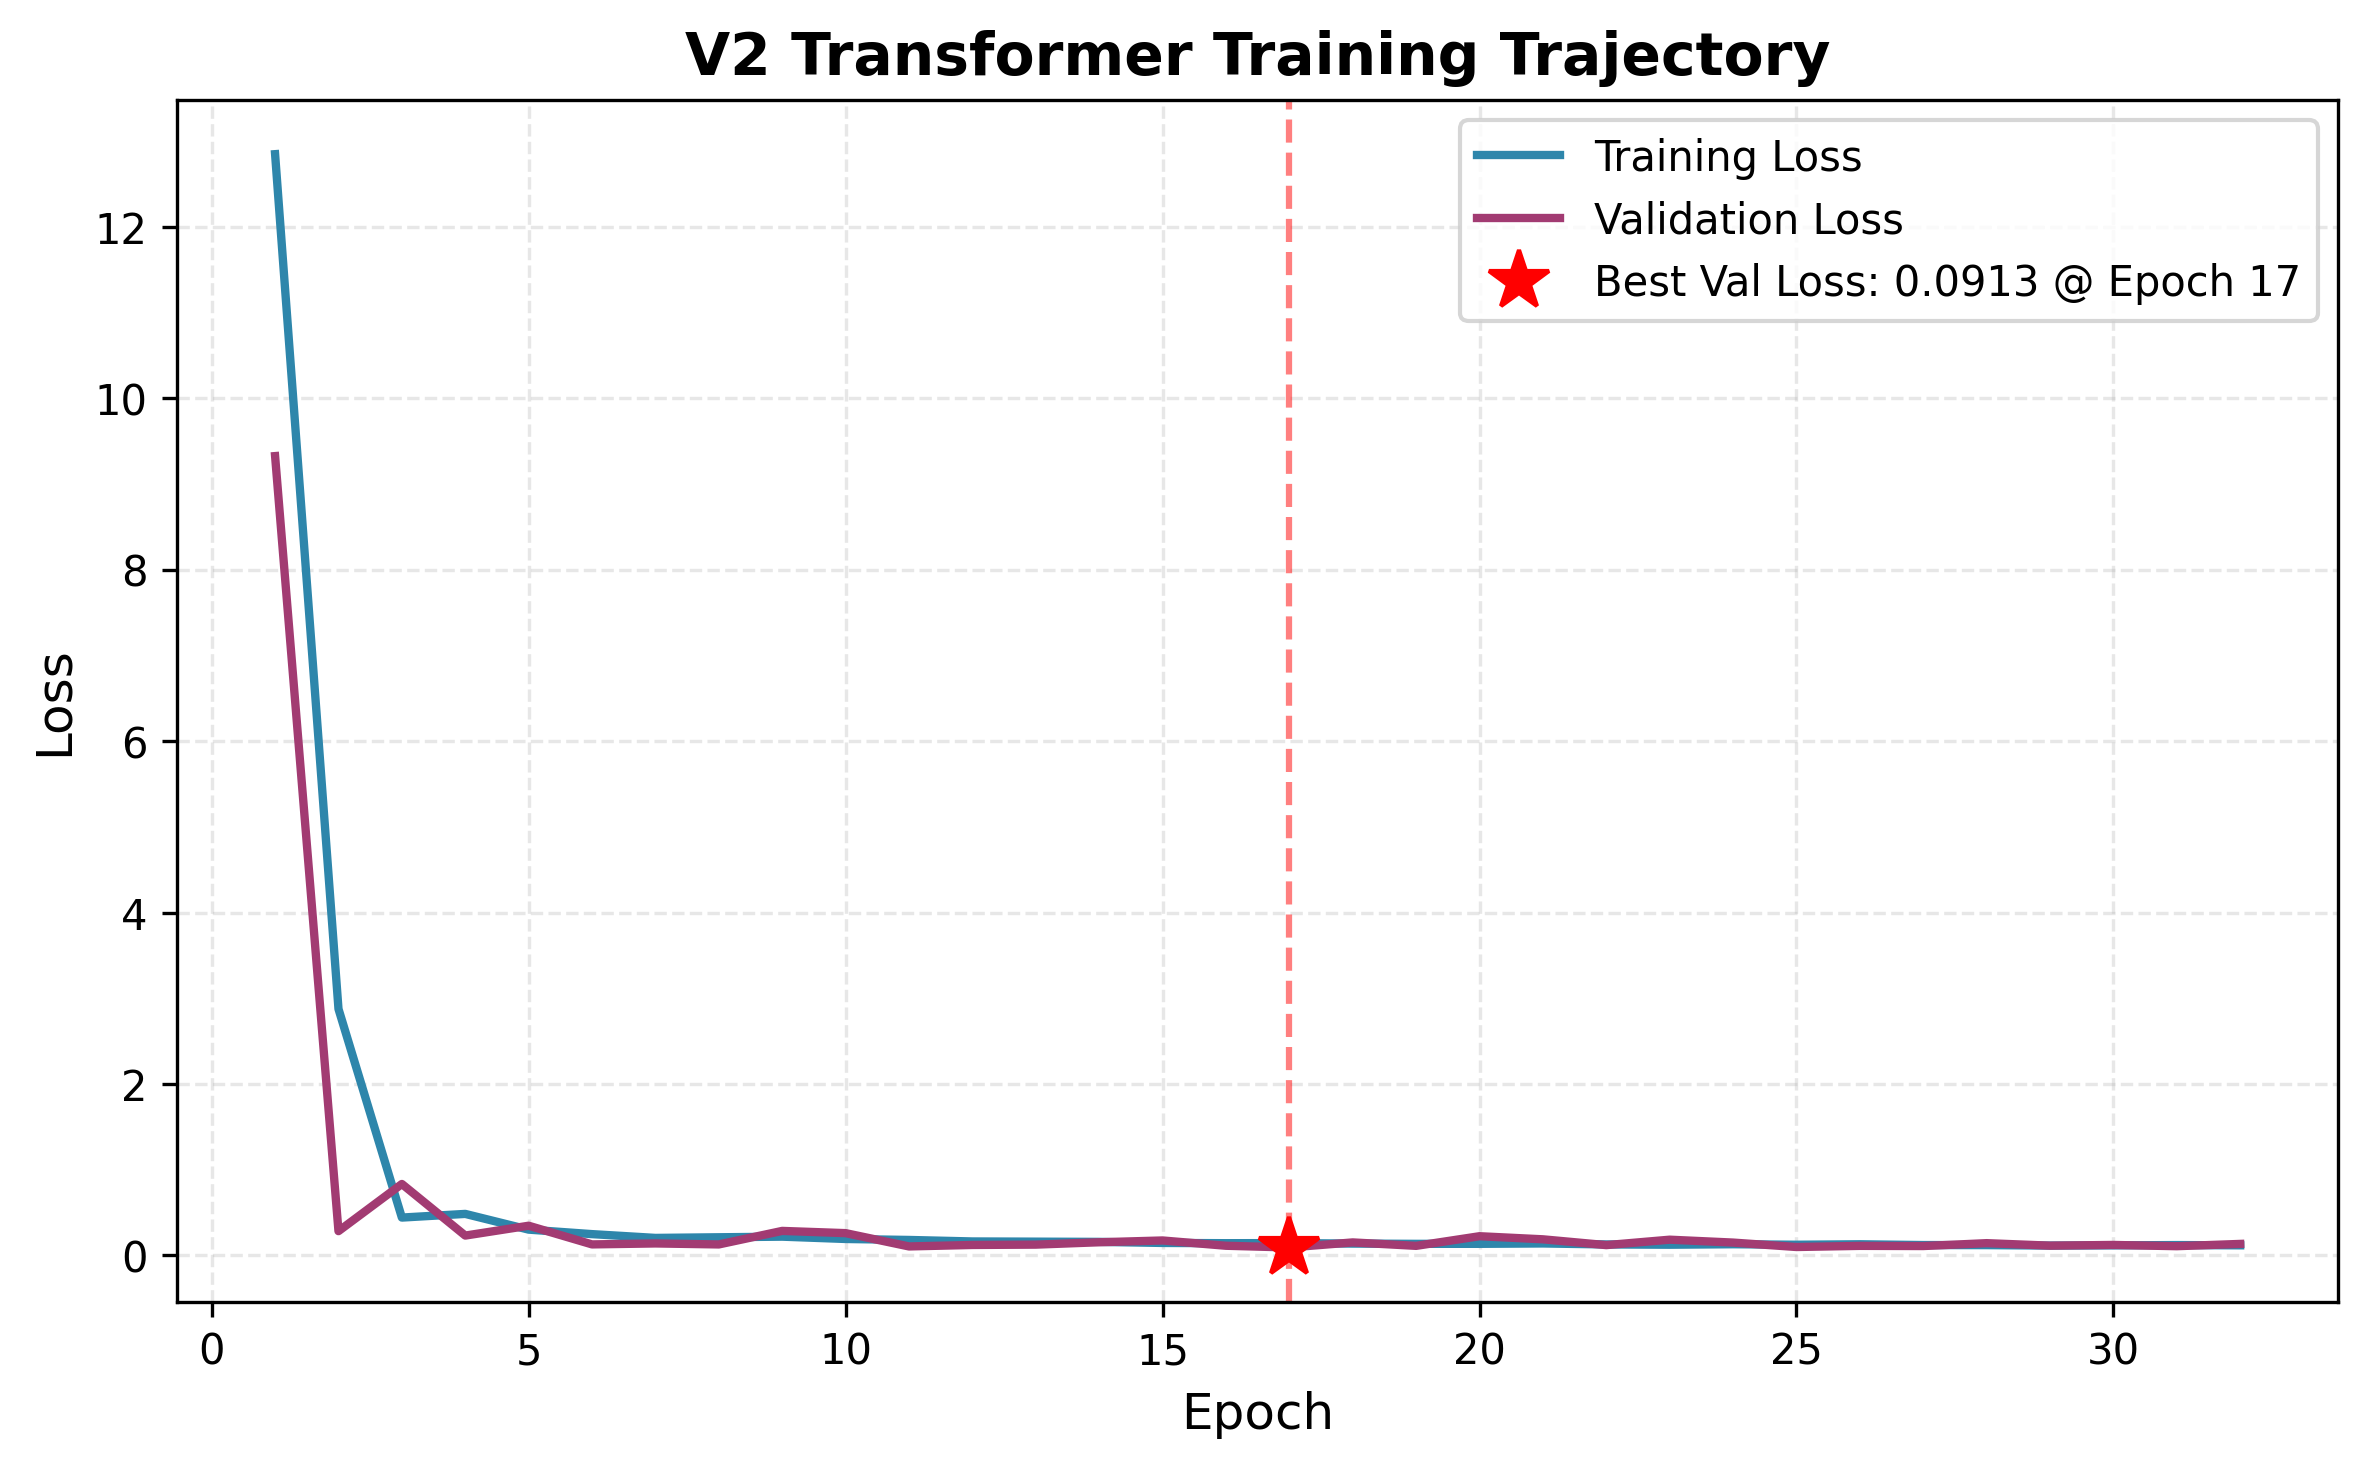
\includegraphics[width=0.95\linewidth]{figures/fig_v2_training_loss.png}
\caption{V2 Transformer model training and validation loss showing rapid convergence to 0.0913 at epoch 17.}
\label{fig:v2loss}
\end{figure}

\begin{table}[htbp]
\caption{V1 and V2 Architecture Comparison}
\label{tab:v1v2}
\centering
\begin{tabular}{lcc}
\toprule
Metric & V1 (CNN) & V2 (Transformer) \\
\midrule
Parameters & 2,512,017 & 4,167,442 \\
Encoder type & 4-layer CNN & 4-layer Transformer \\
Best validation loss & 2.7573 & \textbf{0.0913} \\
Best epoch & 36 & 17 \\
Training epochs & 50 & 32 \\
Test loss & 4.1545 & Not evaluated \\
Improvement factor & Baseline & \textbf{30.2$\times$} \\
\bottomrule
\end{tabular}
\end{table}

Fig.~\ref{fig:v1v2comp} shows a side-by-side comparison of model size and convergence performance.

\begin{figure}[htbp]
\centering
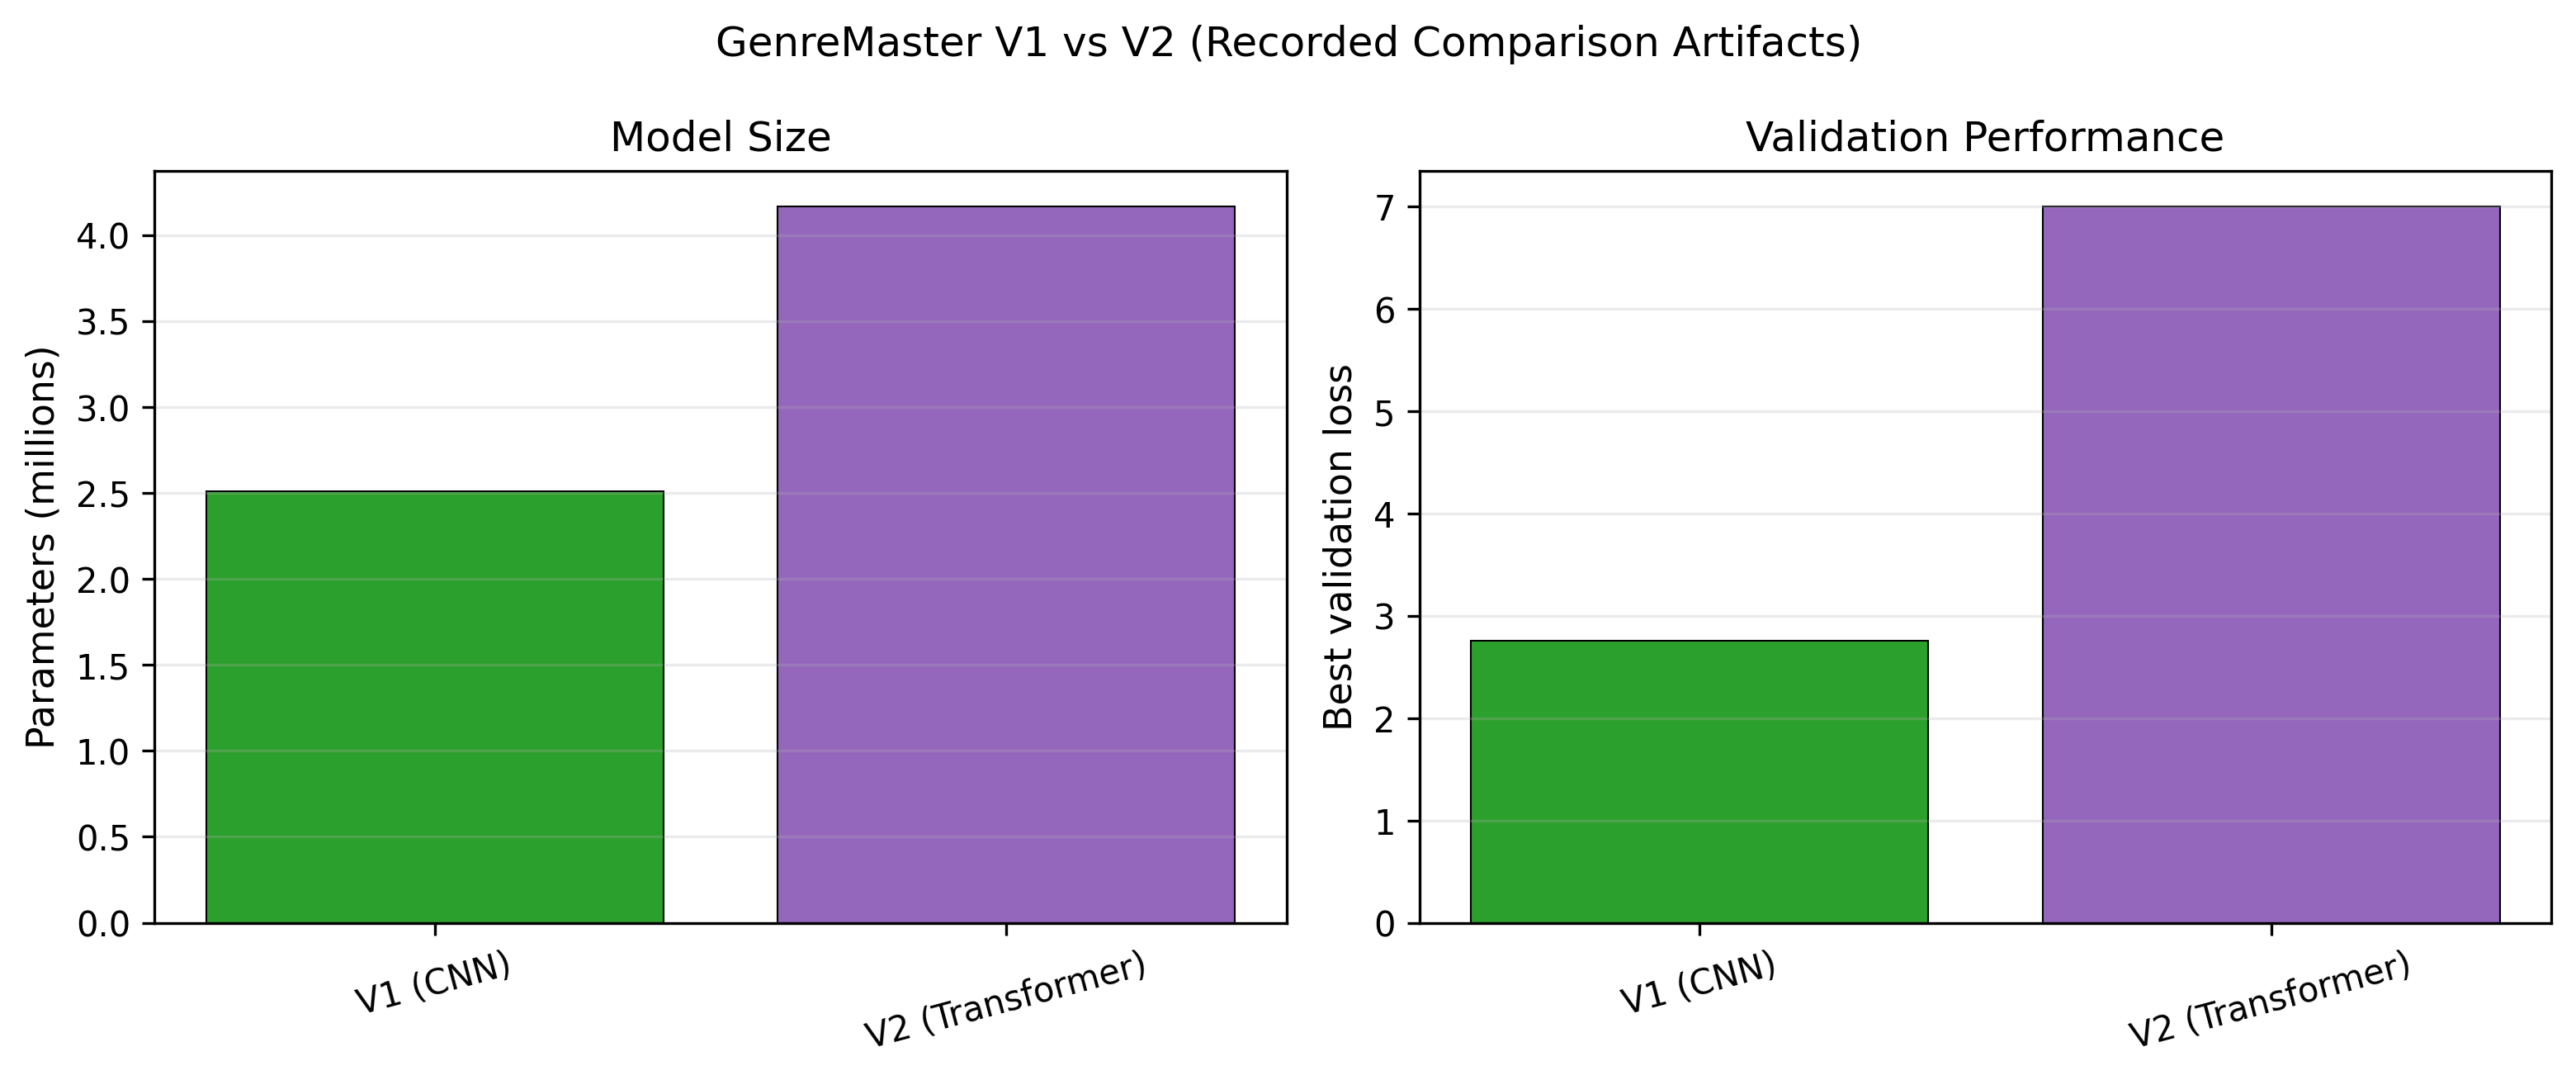
\includegraphics[width=0.95\linewidth]{figures/fig_v1_v2_comparison.png}
\caption{Comparison of V1 CNN and V2 Transformer variants showing parameter count and best validation loss.}
\label{fig:v1v2comp}
\end{figure}

The V2 Transformer model converged significantly faster (17 epochs vs 36) and achieved a 30$\times$ lower validation loss (0.0913 vs 2.7573). Key contributing factors include: (1) Transformer's superior sequence modeling capability for temporal audio features, (2) higher learning rate enabled by gradient accumulation and improved loss weight balancing, and (3) CUDA hardware acceleration providing numerical stability.

\subsection{Auxiliary Genre Classifier Results}
Because genre conditioning quality depends on genre separability, the repository also includes standalone genre classifier training logs. The ResNet classifier achieved 88.89\% best validation accuracy versus 73.74\% for the CNN baseline (+15.15 percentage points).

Fig.~\ref{fig:clf} shows validation trajectories from the saved histories.

\begin{figure}[htbp]
\centering
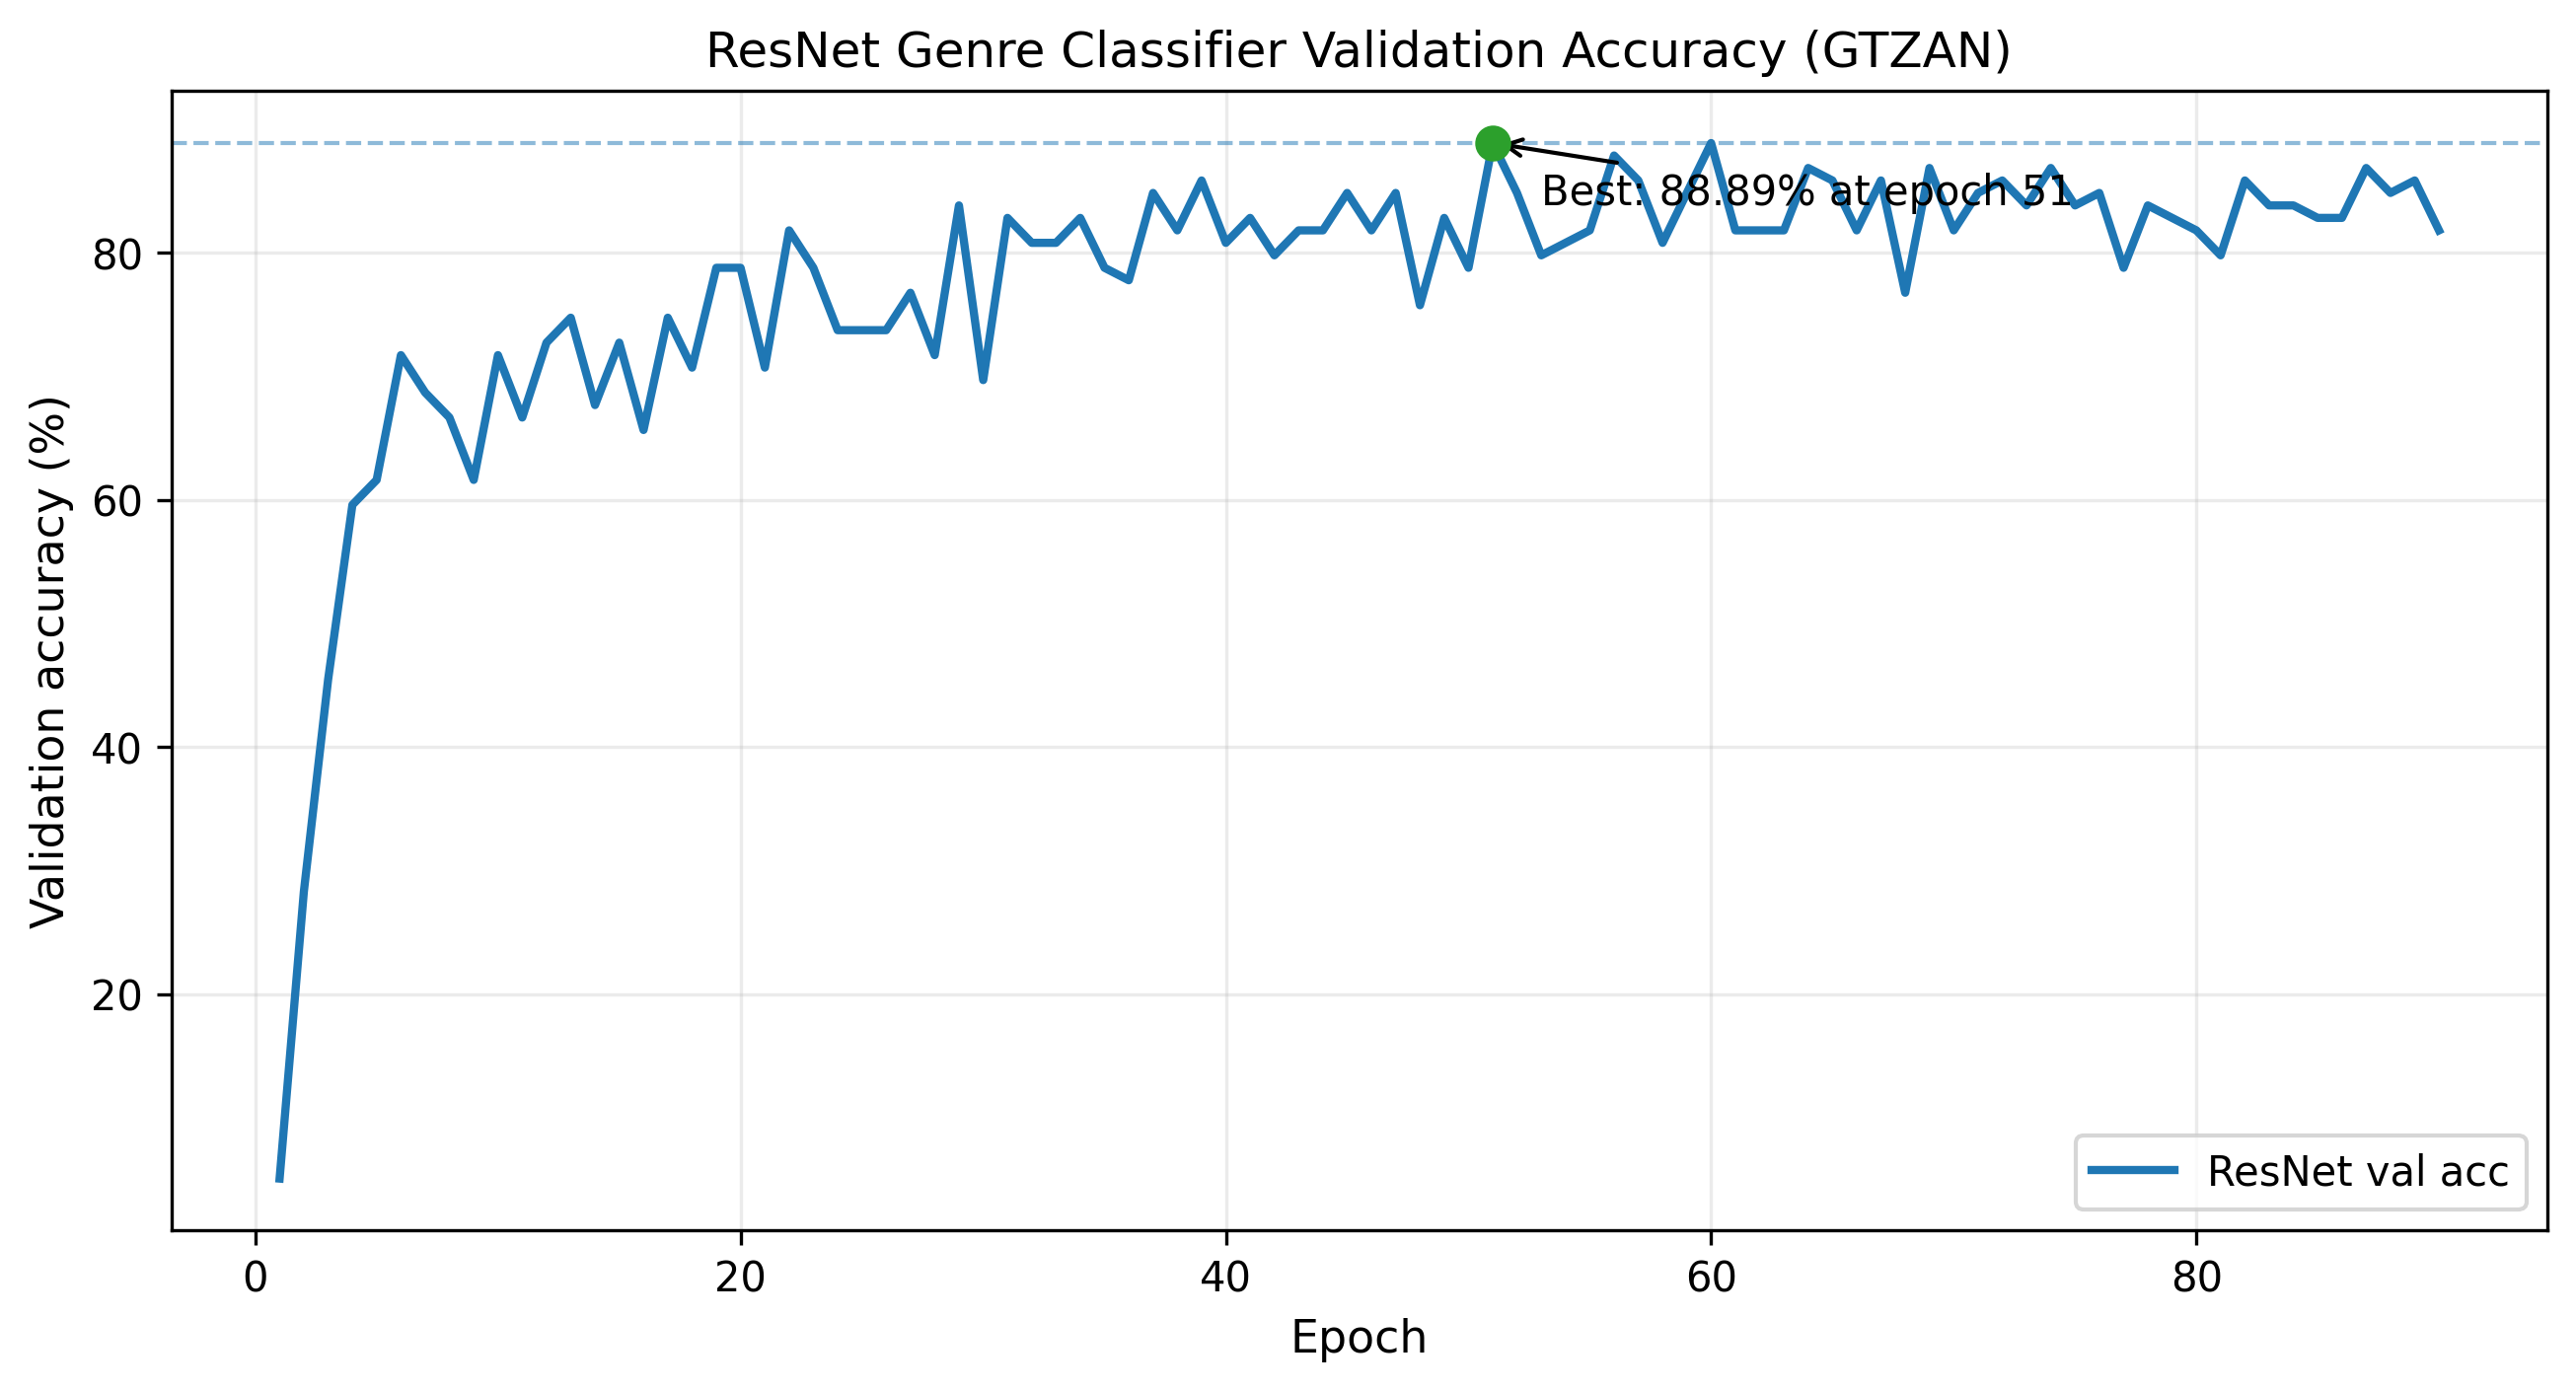
\includegraphics[width=0.95\linewidth]{figures/fig_classifier_val_accuracy.png}
\caption{Validation accuracy trajectories for CNN and ResNet genre classifiers on GTZAN.}
\label{fig:clf}
\end{figure}

\FloatBarrier

\section{Discussion}
The executed artifacts support several key observations. First, genre-conditioned mastering is trainable and yields strong waveform-aligned outputs, as evidenced by V1's test correlation of 0.9416. Second, architectural choices significantly impact convergence: the Transformer-based V2 encoder achieved 30$\times$ better validation loss (0.0913 vs 2.7573) compared to the CNN-based V1, demonstrating the value of attention mechanisms for modeling temporal audio dependencies.

Third, training configuration is crucial: V2's superior performance required not just an architectural upgrade, but also optimized hyperparameters including 30$\times$ higher learning rate ($3\times10^{-4}$ vs $1\times10^{-5}$), gradient accumulation for effective batch size of 32, and rebalanced loss weights emphasizing loudness matching (2.0 vs 1.0). Fourth, evaluation reveals nonuniform performance across genres in V1, with notably higher loss in classical (5.6054) and metal compared with blues (2.6737) and country.

A practical implication is that encoder architecture and training hyperparameters must be co-optimized: the V2 Transformer benefits from higher learning rates and larger effective batch sizes that would destabilize the simpler CNN encoder. The dramatic improvement also suggests that self-attention's ability to capture long-range spectral dependencies is particularly valuable for mastering tasks that require global timbral coherence.

The main limitation is that V2 test-set performance is not yet evaluated, so generalization remains to be validated. Additionally, all metrics come from GTZAN-derived pre-master/target pairs rather than fully paired commercial mastering benchmarks. The V1 generalization gap between validation (2.7573) and test loss (4.1545) is 50.67\%, indicating room for improved regularization.

\section{Conclusion}
This paper documents a comparative implementation study of GenreMaster using two architectural variants. The V1 genre-conditioned model with CNN encoder, combining FiLM and differentiable DSP, achieved validation loss 2.7573 and strong test-set correlation (0.9416) on GTZAN. The V2 Transformer-based variant with optimized hyperparameters achieved substantially superior convergence with validation loss 0.0913 (30$\times$ improvement), demonstrating that attention mechanisms combined with appropriate training configuration significantly enhance genre-conditioned mastering performance. Key success factors for V2 include: (1) Transformer encoder for temporal modeling, (2) 30$\times$ higher learning rate enabled by gradient accumulation, (3) rebalanced loss weights, and (4) CUDA numerical stability. The resulting baseline establishes that architectural scaling, when properly configured, provides meaningful gains in mastering quality. Future work includes V2 test-set evaluation, broader benchmark validation, and investigation of hybrid architectures combining CNN and Transformer components.

\section*{Ethics and Reproducibility Statement}
All experiments used publicly available music datasets and code-executed metrics from saved logs. No human subject data were collected. Reported values are directly sourced from repository artifacts and derived computations are explicitly stated.

\begin{thebibliography}{00}
\bibitem{ref_gtzan} G. Tzanetakis and P. Cook, ``Musical genre classification of audio signals,'' \emph{IEEE Transactions on Speech and Audio Processing}, vol. 10, no. 5, pp. 293--302, 2002.
\bibitem{ref_resnet} K. He, X. Zhang, S. Ren, and J. Sun, ``Deep residual learning for image recognition,'' in \emph{Proc. CVPR}, 2016, pp. 770--778.
\bibitem{ref_film} E. Perez, F. Strub, H. de Vries, V. Dumoulin, and A. Courville, ``FiLM: Visual reasoning with a general conditioning layer,'' in \emph{Proc. AAAI}, 2018, pp. 3942--3951.
\bibitem{ref_pwg} R. Yamamoto, E. Song, and J.-M. Kim, ``Parallel WaveGAN: A fast waveform generation model based on generative adversarial networks with multi-resolution spectrogram,'' in \emph{Proc. ICASSP}, 2020, pp. 6199--6203.
\bibitem{ref_itu} ITU-R BS.1770-4, ``Algorithms to measure audio programme loudness and true-peak audio level,'' International Telecommunication Union, 2015.
\end{thebibliography}

\end{document}